\documentclass[a4paper,12pt]{book}
\usepackage[utf8]{inputenc}
\usepackage{graphicx}
\usepackage{amsmath}
\usepackage{amsfonts}
\usepackage{amssymb}
\usepackage{pgfplots}
\usepgfplotslibrary{fillbetween} % For hatched graphs.
\usetikzlibrary{patterns} % Also for hatched graphs.
\usepackage{subcaption}
% This package is used to mark right-angles. In theory I could have used it more, but it wasn't necessary.
\usepackage{tkz-euclide}
% For underlines and strike-throughs.
\usepackage{ulem}
% For hyperlinks.
\usepackage{hyperref}
\setcounter{tocdepth}{1}
\pgfplotsset{compat=1.16}

\begin{document}

\author{Patrick Ausel}
\title{Higher Mathematics}
\date{2019/2020}

\frontmatter
\maketitle
\tableofcontents

\chapter{Preface}
Because of many things that were supposed to happen in 2020, I decided that it's a better idea to leave this project unfinished. Because of the COVID-19 pandemic the SQA exams were cancelled. There are other resources that have been written, albeit not in such a pretty \LaTeX format, available already which have been tried and tested before; the one that I immediately think of is the \href{https://www.hsn.uk.net/higher-maths/notes/}{Higher Still Notes}\footnote{Available online under \url{https://www.hsn.uk.net/higher-maths/notes/}.}, also written by former Higher Maths students.

That leaves the question, why is this document still up? Well, maybe it'll still be useful for certain pupils, maybe it'll be useful for people wanting to learn \LaTeX. If you wish to finish this, then please feel free to do so! You can fork this repository and do whatever with it, it's licensed under CC0 --- and if you're somehow reading a printed copy and have no idea what I'm talking about, then you can visit \url{https://github.com/TheSheepGuy/Open_Higher_Maths}.

\mainmatter
\chapter{Straight Line}


\section{Gradient \& Equation of a Straight Line}
The gradient is the line's steepness. The bigger the number, the steeper it is. Its symbol is $m$.

Its equation is
\begin{equation*}
m = \frac{\text{vertical distance}}{\text{horizontal distance}}
\end{equation*}
or
\begin{equation}
m = \frac{y_2-y_1}{x_2-x_1}
\end{equation}

If the line is vertical ($\vert$), then it has an undefined gradient, e.g. when $x=1$. If it is horizontal (—), then $m=0$, e.g. when $y=1$.

From National 5, it should be known that, given a point and gradient, the equation of a line can be written using

\begin{equation}
y-b=m(x-a).
\end{equation}

\subsection{Example}
If $m=3$ and the line goes through point (-2,3), find the equation of the line.

\begin{align*}
y-b&=m(x-a)\\
y-3&=3(x+2)\\
y&=3(x+2)+3\\
y&=3x+6+9\\
y&=3x+9\\
\end{align*}

Note that the equation can be left in any form, no extra marks are awarded for leaving it in the form $0 = 3x - y + 9$


\section{$m=\tan\theta$}

\begin{figure}[h!]
	\centering
	\begin{tikzpicture}% function
		\begin{axis}
		[
			xlabel=$x$,
			ylabel=$y$,
			axis lines = left, % Only show axis on the left and bottom.
			axis equal,
			ymin = 0,
			xmin = 0,
		]
		\pgfplotsset{ticks=none}
		\addplot
		[
			samples = 100,
			color = black,
		]{sqrt(3)*x};
		\end{axis}
	\end{tikzpicture}
	\caption{Here, $\theta$ is 60$^\circ$.}
	\label{fig:mtan60}
\end{figure}
$\theta$ is the (in figure \ref{fig:mtan60} an acute) angle made from the $x$-axis in an anti-clockwise direction (also called in the positive direction of the $x$-axis). If $\theta$ is known, the gradient of the line can be found, and vice versa, by using

\begin{equation}
	m=\tan\theta
\end{equation}

\subsection{Examples}
\begin{enumerate}
	\item
	A line makes an angle of 120$^\circ$ with the positive direction of the $x$-axis. Find its gradient.
	
	One could just enter 120$^\circ$ into their calculator and get the right answer, but the following is a method of working it out if the question would appear in a non-calculator paper.
	\begin{align*}
	m&=\tan\theta\\
	&=\tan120^\circ\\
	&=-\tan60\\
	&=-\sqrt{3}
	\end{align*}
	
	\item
	A line's gradient is $-2$. Find the angle it makes in the positive direction of the $x$-axis.
	\begin{align*}
	\text{If $m=2$,}\\
	\tan\theta&=2\\
	\theta&=\tan^{-1}2\\
	&=63.43...\\
	\text{Now the proper line where $m=-2$,}\\
	\theta&=180-63.43...\\
	&=116.56...\\
	&\approx116.6^\circ
	\end{align*}

\end{enumerate}


\section{Perpendicular Lines ($\perp$)}
Perpendicular lines sit at right angles to each other. If lines are perpendicular, then
\begin{equation}
m_1 m_2 = -1.
\end{equation}

\subsection{Examples}
If two lines are perpendicular, calculate $m_1$ if $m_2$ is
\begin{enumerate}
	\item 6
	\item -7
	\item $\frac{2}{7}$
\end{enumerate}

\begin{enumerate}
	\item
	\begin{align*}
	m_1 m_2 &= -1\\
	3m_1 &= -1\\
	m_1&=-\frac{1}{3}
	\end{align*}
	
	\item
	\begin{align*}
	m_1 m_2 &= -1\\
	-7m_1 &= -1\\
	m_1&=\frac{1}{7}
	\end{align*}
	
	\item
	\begin{align*}
	m_1 m_2 &= -1\\
	\frac{2}{7}m_1 &= -1\\
	2m_1&=-7\\
	m_1&=-\frac{7}{2}
	\end{align*}
\end{enumerate}

As a shortcut, take the recipricol and change the sign.

\begin{enumerate}
	\setcounter{enumi}{3}
	\item
	Find the equation of the line perpendicular to $y=-\frac{2}{3}x+5$ that passes through the point $\left(1,7\right)$.

	\begin{align*}
		m &= -\frac{2}{3} & m_\perp &= \frac{3}{2}
	\end{align*}

	Now that the gradient of the perpendicular line has been found, it can be used in the equation.
	
	\begin{align*}
		y-b&=m(x-a)\\
		y-7&=\frac{3}{2}(x-1)\\
		y&=\frac{3}{2}x - \frac{3}{2} + 7\\
		y&=\frac{3}{2}x + \frac{11}{2}
	\end{align*}
\end{enumerate}


\section{Mid Point Formula}
To find the point in the middle of a line, use
\begin{equation}
\text{mid point} = \left(\frac{x_1 + x_2}{2},\frac{y_1 + y_2}{2}\right)
\end{equation}

\subsection{Examples}
\begin{enumerate}
	\item
	Find the mid point of $\left(1,-4\right)$ and $\left(7,8\right)$.
	
	\begin{align*}
		\text{mid point} &= \left(\frac{x_1 + x_2}{2},\frac{y_1 + y_2}{2}\right)\\
		&= \left(\frac{1 + 7}{2},\frac{-4 + 8}{2}\right)\\
		&= \left(4,2\right)
	\end{align*}
	
	\item
	A circle has centre point $(6,10)$. Two points $A(5,5)$ and $B$ are drawn on its circumference, these are connecting by a diameter (see figure \ref{fig:MidPointQ2}). Find the coordinates of B.
	\begin{figure}[h!]
		\centering
		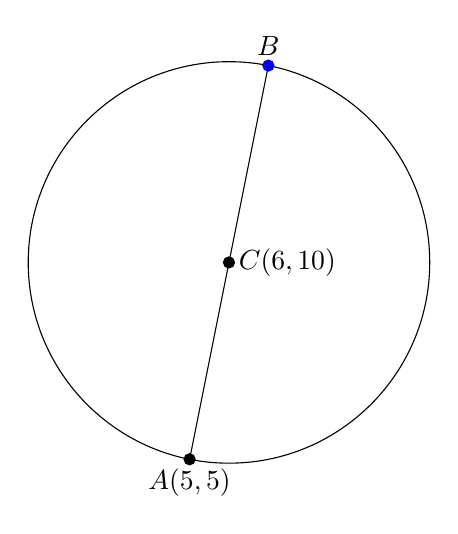
\begin{tikzpicture}
		[
			scale=0.5,
			% Make a style for a black coordinate.
			cmark/.style={label={[anchor=center, color=black]:\pgfuseplotmark{#1}}},
			% And one for a blue coordinate.
			bmark/.style={label={[anchor=center, color=blue]:\pgfuseplotmark{#1}}}
		]
			\draw (6,10) circle [radius=sqrt(26)];
			\coordinate
			[
				label=below:{$A(5,5)$},
				black,
				cmark=*,
			] (a) at (5,5);
			\coordinate
			[
				label=right:{$C(6,10)$},
				black,
				cmark=*,
			] (c) at (6,10);
			\coordinate
			[
				label=above:{$B$},
				blue,
				bmark=*,
			] (b) at (7,15);
			
			% Draw diameter.
			\draw (a) -- (c) -- (b);
		\end{tikzpicture}
		\caption{Circle mentioned in example 2.}
		\label{fig:MidPointQ2}
	\end{figure}
	\begin{align*}
		\text{mid point} &= \left(\frac{x_1 + x_2}{2},\frac{y_1 + y_2}{2}\right)\\
		\left(17, 12\right) &= \left(\frac{9+x}{2},\frac{-2 + y_2}{2}\right)
	\end{align*}
	\begin{align*}
		\frac{9+x}{2} &= 17 & \frac{-2+y}{2} &= 12\\
		9+x &= 34 & -2+y &= 24\\
		x &= 25 & y &= 26
	\end{align*}
	
	So the coordinate of B is $\left(25,26\right)$.
\end{enumerate}


\section{Collinearity}
Points that are collinear lie on a straight line.

\begin{figure}[h!]
	\centering
	\begin{subfigure}[b]{0.4\linewidth}
		\begin{tikzpicture}% coordinates
			\begin{axis}
			[
				axis equal,
				axis line style={draw=none},
			]
			\pgfplotsset{ticks=none} % Get rid of numbers and ticks.
			\addplot
			[
				color=black,
				mark=*,
			] coordinates
			{
				(3,0)(6,1)(9,2)
			};
		\end{axis}
		\end{tikzpicture}
		\caption{Collinear.}
	\end{subfigure}
	\begin{subfigure}[b]{0.4\linewidth}
		\begin{tikzpicture}% coordinates
			\begin{axis}
			[
				axis equal,
				axis line style={draw=none},
			]
			\pgfplotsset{ticks=none} % Get rid of numbers and ticks.
			\addplot
			[
				color=black,
				mark=*,
			] coordinates
			{
				(1,0)(2,1)(7,2)
			};
			\end{axis}
		\end{tikzpicture}
		\caption{Not collinear.}
	\end{subfigure}
	\caption{Examples of collinearity.}
	\label{fig:collinearityExample}
\end{figure}

To test for collinearity of three points $A,B,C$:
\begin{enumerate}
	\item find $m_{AB}$,
	\item find $m_{BC}$,
	\item if $m_{AB}=m_{BC}$, then (because $B$ is a common point) they are collinear.
\end{enumerate}

\subsection{Examples}
\begin{enumerate}
	\item
	Show that the points $P\left(-6,-1\right), Q\left(0,2\right), R\left(8,6\right)$ are collinear.
	
	\begin{align*}
		m_{PQ}&=\frac{2+1}{0+6} & m_{QR}&=\frac{6-2}{8-0}\\
		&=\frac{3}{6} & &=\frac{4}{8}\\
		&=\frac{1}{2} & &=\frac{1}{2}
	\end{align*}
	Since $m_{PQ} = m_{QR}$, and $Q$ is a common point, $PQR$ are collinear.
	
	\item
	If $A\left(1,-1\right), B\left(-1,k\right), C\left(5,7\right)$ are collinear, find k.
	
	\begin{align*}
		m_{AB}&=m_{BC}\\
		\frac{k-(-1)}{-1-1}&=\frac{7-k}{5-(-1)}\\
		\frac{k+1}{-2}&=\frac{7-k}{6}\\
		6(k+1)&=-2(7-k)\\
		6k+6&=-14+2k\\
		4k&=-20\\
		k&=5
	\end{align*}
\end{enumerate}


\section{Median Lines}
\begin{figure}[h!]
	\centering
	\begin{tikzpicture}[scale=8]
		% Draw triangle.
		\coordinate[label=left:{$A$}] (a) at (0mm,0mm);		\coordinate[label=above:{$B$}] (b) at (7mm,5mm);		\coordinate[label=right:{$C$}] (c) at (10mm,1mm);
		\draw (a) -- (b) -- (c) -- cycle;
		
		% Draw point M.
		\coordinate
		[
			label=below:{$M$},
			circle,
			fill,
			color=blue,
			inner sep=1mm,
			scale=0.5
		] (m) at (5mm,0.5mm);
		
		% Connect point M and B.
		\draw[color=blue] (m) -- (b) -- cycle;
	\end{tikzpicture}
	\caption{Median from B.}
	\label{fig:median}
\end{figure}

The median is a line from a vertex of a triangle to the mid point of the opposite.

To find the median from $B$ in a triangle $ABC$ (such as in figure \ref{fig:median}):
\begin{enumerate}
	\item find the mid point of $AC$ (hereafter called $M$), since the opposite of $B$ is $AC$,
	\item find $m_{BM}$,
	\item use $y-b=m(x-a)$ with $B$ or $M$ and $m_{BM}$.
\end{enumerate}

\subsection{Example}
In $\triangle ABC$, $A(4,-9)$, $B(10,2)$, and $C(4,-4)$. Find the equation of the median from A.

\begin{align*}
	\text{mid point} &= \left(\frac{10+4}{2},\frac{2-4}{2}\right) & m_{AM} &= \frac{-1-(-9)}{7-4}\\
	&=\left(7,-1\right) & &= \frac{8}{3}
\end{align*}
\begin{align*}
	y-b&=m(x-a)\\
	y+9&=\frac{8}{3}\left(x-4\right)\\
	3y+27&=8\left(x-4\right)\\
	3y&=8x-32-27\\
	3y&=8x-59
\end{align*}


\section{Altitude}
\begin{figure}[h!]
	\centering
	\begin{tikzpicture}[scale=2]
		% Draw triangle.
		\coordinate[label=left:{$A$}] (a) at (0cm,0cm);		\coordinate[label=above:{$B$}] (b) at (1cm,2.5cm);		\coordinate[label=right:{$C$}] (c) at (2.5cm,0.5cm);
		\coordinate[] (q) at ($(c)!(b)!(a)$) {};
		\draw (a) -- (b) -- (c) -- cycle;
		\draw[color=blue] (b) -- (q);
		
		\tkzMarkRightAngle[radius=0.05cm](b,q,c)
	\end{tikzpicture}
	\caption{Altitude from B.}
	\label{fig:altitude}
\end{figure}

The altitude is a straight line from a vertex to the other side at right angles.

To find the altitude from $B$ in a triangle $ABC$ (such as in figure \ref{fig:altitude}):
\begin{enumerate}
	\item find $m_{AC}$,
	\item find $m_\perp$,
	\item use $y-b=m(x-a)$ with $m_\perp$ and $B$.
\end{enumerate}

\subsection{Example}
The triangle $ABC$ has vertices $A(3,-5)$, $B(4,3)$, and $C(-7,2)$. Find the altitude from A.

\begin{align*}
	m_{CB}&=\frac{3-2}{4-(-7)} & m_\perp&=-11\\
	&=\frac{1}{11}
\end{align*}
\begin{align*}
	y-b&=m(x-a)\\
	y+5&=-11(x-3)\\
	y&=-11x+33-5\\
	y&=-11x+28
\end{align*}


\section{Perpendicular Bisector}
\begin{figure}[h!]
	\centering
	\begin{tikzpicture}[scale=2]
		% Draw triangle.
		\coordinate[label=above:{$A$}] (a) at (0cm,0cm);
		\coordinate[label=above:{$B$}] (b) at (4cm,0cm);
		\coordinate[] (p) at (2cm,0.75cm);
		\coordinate[] (q) at (2cm,0cm);
		\coordinate[] (r) at (2cm,-0.75cm);
		\draw (a) -- (b);
		\draw[color=blue] (p) -- (r);
		
		\tkzMarkRightAngle[radius=0.05cm](p,q,b)
	\end{tikzpicture}
	\caption{The perpendicular bisector of $AB$ is here in blue.}
	\label{fig:pb}
\end{figure}

The perpendicular bisector (abbr. PB) is a line that cuts another line in the middle and sits at right angles.

To find the PB of a line $AB$:
\begin{enumerate}
	\item find the mid point $AB$,
	\item find $m_{AB}$,
	\item find $m_\perp$,
	\item use $y-b=m(x-a)$ with the mid point $AB$ and $m_\perp$.
\end{enumerate}

\subsection{Example}
Two points are $A(-2,1)$ and $B(4,7)$ are connected by a line. Find the equation of the perpendicular bisector.

\begin{align*}
	\text{mid point} &= \left(\frac{-2+4}{2},\frac{1+7}{2}\right) & m_{AB} &= \frac{7-1}{4-(-2)} & m_\perp&=-1\\
	&=(1,4) & &=1
\end{align*}
\begin{align*}
	y-b&=m(x-a)\\
	y-4&=-1(x-1)\\
	y&=-x+1+4\\
	y&=-x+5
\end{align*}

\begin{figure}[h!]
	\centering
	\begin{tikzpicture}
	[
		scale=0.5,
		% Make a style for a black coordinate.
		cmark/.style={label={[anchor=center, color=black]:\pgfuseplotmark{#1}}},
		% And one for a blue coordinate.
		bmark/.style={label={[anchor=center, color=blue]:\pgfuseplotmark{#1}}}
	]
		\coordinate
		[
			label=left:{$A(-2,1)$},
			black,
			cmark=*,
			] (a) at (-2,1);
		\coordinate
		[
			label=right:{$B(4,7)$},
			black,
			cmark=*,
		] (b) at (4,7);
		\coordinate (p) at (0,5);
		\coordinate [label=right:{$y=-x+5$}] (q) at (2,3);
		
		% Draw line
		\draw (a) -- (b);
		\draw[blue] (p) -- (q);
	\end{tikzpicture}
	\caption{Perpendicular bisector in blue. Note that this is only to show what's happening, it's not required to sketch this in an exam unless specifically asked for.}
	\label{fig:PBexample}
\end{figure}


\section{Intersection of Lines}
The point of intersection (abbr. POI) of two lines can be found through solving each line's equation simultaneously.

The National 5 course most likely focussed on the method of elimination, a better method is to use substitution. However, sometimes, such as in the second example, the equations are so simple that it would be stupid to not eliminate.

\subsection{Examples}
\begin{enumerate}
	\item
	Two lines have equations $2x-y+11=0$ and $x+2y-7 = 0$. Find the point of intersection.
	
	\begin{align*}
		2x-y+11&=0\\
		y&=2x+11
	\end{align*}
	Sub $y=2x+11$ into $x+2y-7=0$,
	\begin{align*}
		x+2(2x+11)-7&=0\\
		x+4x+22-7&=0\\
		5x+15&=0\\
		5x&=-15\\
		x&=-3
	\end{align*}
	\begin{align*}
		y&=2x+11 & POI=(-3,5)\\
		y&=2(-3)+11\\
		&=-6+11\\
		&=5
	\end{align*}
	\begin{figure}[h!]
		\centering
		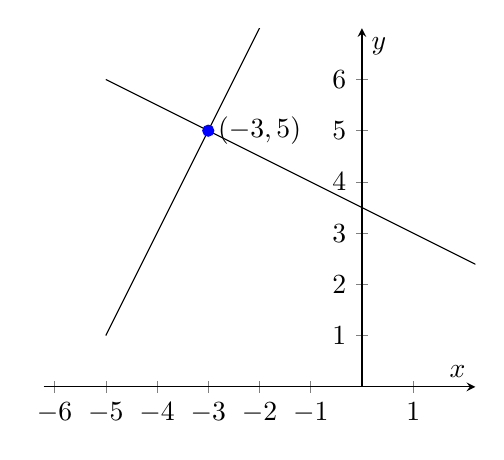
\begin{tikzpicture}[bmark/.style={label={[anchor=center, color=blue]:\pgfuseplotmark{#1}}}]
			\begin{axis}
			[
				xlabel=$x$,
				ylabel=$y$,
				xmin=-6,
				xmax=2,
				xtick={-6,-5,...,1},
				ymin=0,
				ymax=7,
				ytick={0,1,...,6},
				axis lines=center,
				axis equal,
				smooth,
				scale=0.8,
			]
				\addplot [color=black,mark=none] {2*x+11};
				\addplot [color=black,mark=none] {3.5-0.5*x};
				\coordinate
				[
					label=right:{$(-3,5)$},
					bmark=*,
				] (a) at (-3,5);
			\end{axis}
		\end{tikzpicture}
		\caption{Solution to the first example, point of intersection in blue. Again, it's not required to sketch these two lines, this figure is simply there to give further clarification as to what's happening.}
		\label{fig:POIexample}
	\end{figure}
	
	\item
	In triangle $ABC$ with points $A(1,0)$, $B(-4,3)$, $C(0,-1)$, find the median from A, the altitude from C, and henceforth the POI.
	
	\textit{Median from A:}
	\begin{align*}
		\text{mid point} &= \left(\frac{-4+0}{2},\frac{3+(-1)}{2}\right) & m &= \frac{3-0}{-4-1} \\
		&= (-2,1) & &=-\frac{1}{3}
	\end{align*}
	\begin{align*}
		y-b&=m(x-a)\\
		y-1&=-\frac{1}{3}\left(x+2\right)\\
		3y-3&=-\left(x+2\right)\\
		3y&=-x-2+3\\
		3y&=-x+1
	\end{align*}
	
	\textit{Altitude from C:}
	\begin{align*}
		m_{AB}&=\frac{3-0}{-4-1} & m_\perp&=\frac{5}{3} \\
		&=-\frac{3}{5}
	\end{align*}
	\begin{align*}
		y-b&=m(x-a)\\
		y+1&=\frac{5}{3}\left(x+0\right)\\
		3y+3&=5\left(x+0\right)\\
		3y&=5x-3
	\end{align*}
	
	\textit{Point of intersection:}
	\begin{align*}
		3y&=-x+1 & 3y&=-x+1\\
		\makebox[0pt][l]{\uline{\phantom{$--3y=5x-3$}}}
		-\;\;3y&=5x-3 & 3y&=-\frac{2}{3}+1\\
		0&=-6x+4 & 9y&=-2+3\\
		6x&=4 & 9y&=1\\
		x&=\frac{2}{3} & y=\frac{1}{9}\\
	\end{align*}
	\begin{equation*}
		POI = \left(\frac{2}{3},\frac{1}{9}\right)
	\end{equation*}
\end{enumerate}

% Define number set symbols.
\newcommand{\N}{\mathbb{N}}
\newcommand{\Z}{\mathbb{Z}}
\newcommand{\Q}{\mathbb{Q}}
\newcommand{\R}{\mathbb{R}}
\newcommand{\C}{\mathbb{C}}

\chapter{Functions and Graphs}
\section{Composite Functions}
A function $f(x) = 3x+9$ will take in any value for $x$, and substitutes it into the expression $3x+9$. If another expression would be passed into $f(x)$, such as $x-2$, then the result would be $3(x-2)+9$. A composite function is one where two functions are combined, similar to above.

Suppose $f(x) = 2x$ and $g(x) = x+1$, then composite functions $f(g(x))$ and $g(f(x))$ can be found as follows:
\begin{align*}
	f(g(x)) &= 2(x+1) & g(f(x)) &= (2x)+1\\
	&=2x+2 & &=2x+1
\end{align*}

A composite function can get tiring to write out all the time. So it could be written as $h(x)=f(g(x))$.

\subsection{Example}
$f(x)=x^2+1$ and $g(x)=\frac{1}{x} \left(x\neq0\right)$. Find $h(x)=f(g(x))$ and $h(x)=g(f(x))$.
\begin{align*}
	h(x)&=f\left(\frac{1}{x}\right) & k(x)&=g\left(x^2+1\right)\\
	&=\left(\frac{1}{x}\right)^2-2 & &=\frac{1}{x^2+1}\\
	&=\frac{1}{x^2}-1
\end{align*}


\section{Domains and Set Notation}
A function most often can't take all numbers as inputs. For example, a function of the area of a rectangle might be written as $f(x)=x^2+2x-8$. Since it's a function of real-life area in terms of lengths, the area cannot be negative. After some thinking, it can be concluded that $x$ must be 2 or larger. So the function's domain is any number larger or equal to 2.

Additionally, a real number (aka decimal number) could also be passed in to the function, but maybe that's not what you want. You can also define the domain to only include natural numbers (positive whole numbers).

Applying these two factors, the domain of the function is $\{x \in \N \mid x \geq 2\}$

Set (or rather set-builder) notation is a way of describing a set of numbers. In relation to domains, it details what set of numbers can be an acceptable input of the function. The kinds of set number symbols that exist commonly are
\begin{itemize}
	\item $\N$, natural numbers. Non-negative integers (so starting with 0, counting up in steps of 1).
	\item $\Z$, integers. Any number that can be written without a fractional component (``whole" numbers).
	\item $\Q$, rational numbers. A number which can be written as a fraction with an integer numerator and a non-zero natural denominator\footnote{Negative denominators can exist, but are avoided, as they can be expressed as a negative numerator instead.}.
	\item $\R$, real numbers. Any number that can be represented on a number line.
\end{itemize}

\subsection{Example}
Find a suitable domain for the function $\frac{1}{x^2-1}$.

\begin{equation*}
	\{x \in \R \mid x \neq \sqrt{2}\}
\end{equation*}


\section{Inverse Functions}
An inverse function ($f^{-1}(x)$) will do the opposite as what its normal counterpart ($f(x)$) does. For example,
\begin{align*}
	f(x) &= x^2\\
	f^{-1}(x)&=\sqrt{x}
\end{align*}

Functions are said to be inverse if $f\left(f^{-1}(x)\right) = f^{-1}\left(f(x)\right)=x$.

A trick for finding the inverse of a function is to do the following:
\begin{enumerate}
	\item replace $f(x)$ with $y$,
	\item change the subject of the formula for $x$,
	\item change $y$ to $x$, and $x$ to $f^{-1}(x)$.
\end{enumerate}

\subsection{Examples}
\begin{enumerate}
	\item
	\begin{align*}
		f(x)&=2x\\
		y&=2x\\
		x&=\frac{y}{2}\\
		f^{-1}(x)&=\frac{x}{2}
	\end{align*}
	\item
	\begin{align*}
		f(x)&=2x+1\\
		y&=2x+1\\
		2x&=y-1\\
		x&=\frac{1}{2}\left(y-1\right)\footnotemark\\
		f^{-1}(x)&=\frac{1}{2}\left(x-1\right)
	\end{align*}
	\footnotetext{Note that writing $x=\frac{y-1}{2}$ is correct too. That means that $f^{-1}(x)=\frac{x-1}{2}$ is a perfectly acceptable answer.}
\end{enumerate}


\section{Graph of $y=f(x)+a$ and \dots$-a$}
Given a graph $y=f(x)$, if asked to sketch $y=f(x)+a$, the graph would be moved $a$ places up; if asked to sketch $y=f(x)-a$, the graph would be moved $a$ places down.

In other words, the graph is moved $a$ places along the $y$-axis. A value of $-3$ would move the graph $-3$ places up (i.e. $3$ places down). Practically, add $a$ to all $y$-coordinates.

\subsection{Example}
In figure \ref{fig:verticalShiftExample}, the original graph $y=f(x)$ is drawn, along with $y=f(x)+3$.

\begin{figure}[h!]
	\centering
	\begin{subfigure}{0.475\linewidth}
		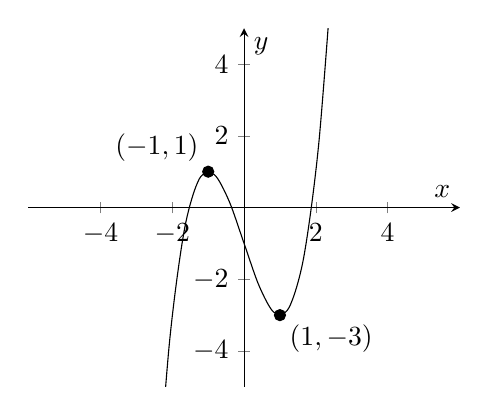
\begin{tikzpicture}[cmark/.style={label={[anchor=center]:\pgfuseplotmark{#1}}}]
			\begin{axis}
			[
				restrict y to domain=-10:10,
				restrict x to domain=-5:5,
				xlabel=$x$,
				ylabel=$y$,
				xmin=-5,
				xmax=5,
				xtick={-4,-2,...,4},
				ymin=-5,
				ymax=5,
				ytick={-4,-2,...,3},
				axis lines=center,
				axis equal,
				smooth,
				scale=0.8
			]
				\addplot [] {x^3-3*x-1};
				\coordinate
				[
					label=above left:{$(-1,1)$},
					black,
					cmark=*,
				] (a) at (-1,1);
				\coordinate
				[
					label=below right:{$(1,-3)$},
					black,
					cmark=*,
				] (a) at (1,-3);
			\end{axis}
		\end{tikzpicture}
		\caption{Some function $y=f(x)$ with a couple of given coordinates.}
	\end{subfigure}
	\begin{subfigure}{0.475\linewidth}
		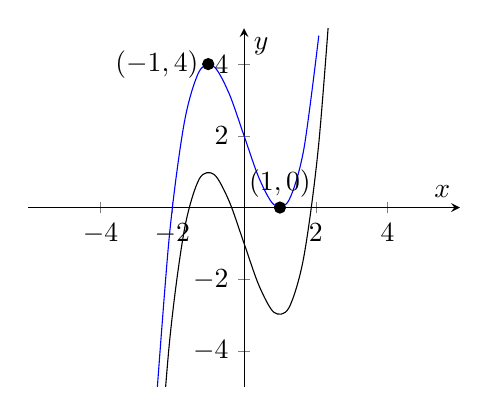
\begin{tikzpicture}[cmark/.style={label={[anchor=center]:\pgfuseplotmark{#1}}}]
			\begin{axis}
			[
				restrict y to domain=-10:10,
				restrict x to domain=-5:5,
				xlabel=$x$,
				ylabel=$y$,
				xmin=-5,
				xmax=5,
				xtick={-4,-2,...,4},
				ymin=-5,
				ymax=5,
				ytick={-4,-2,...,3},
				axis lines=center,
				axis equal,
				smooth,
				scale=0.8
			]
				\addplot [mark=none] {x^3-3*x-1};
				\addplot [color=blue,mark=none] {x^3-3*x+2};
				\coordinate
				[
					label=left:{$(-1,4)$},
					black,
					cmark=*,
				] (a) at (-1,4);
				\coordinate
				[
					label=above:{$(1,0)$},
					black,
					cmark=*,
				] (a) at (1,0);
			\end{axis}
		\end{tikzpicture}
		\caption{$y=f(x)+3$ in blue, along with the original graph.}
	\end{subfigure}
	\caption{An example of a typical question about $y=f(x)+a$ with the solution.}
	\label{fig:verticalShiftExample}
\end{figure}

To find out the transformed coordinates, add $a$ to the $y$-coordinates:
\begin{align*}
f(x)&=(-1,1) & f(x)&=(1,-3)\\
f(x)+3&=(-1,4) & f(x)+3&=(1,0)
\end{align*}


\section{Graph of $y=f(x+a)$ and \dots$-a)$}
When the $a$ is inside the bracket, it moves the graph from side to side. A graph of $y=f(x+a)$ will move the graph $a$ places \textit{left}, and $y=f(x-a)$ would move $a$ places \textit{right}.

In other words, the graph is moved $-a$ places along the $x$-axis. A value of $-3$ would move the graph 3 places to the right. Practically, add $-a$ to all $x$-coordinates. The thing to throw you off is that it is $-a$, and not $a$ that is being moved.

\subsection{Example}
The figure \ref{fig:horizontalShiftExample} is the graph $y=f(x)$ and $y=f(x+5)$.

\begin{figure}[h!]
	\centering
	\begin{subfigure}{0.475\linewidth}
		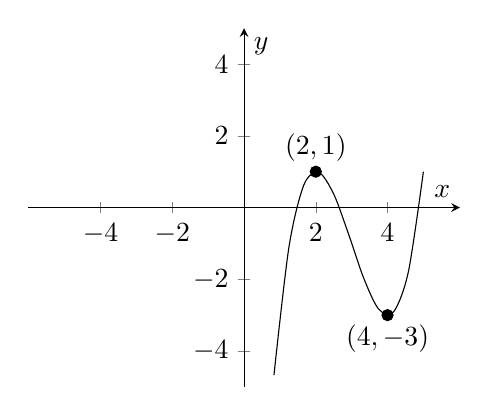
\begin{tikzpicture}[cmark/.style={label={[anchor=center]:\pgfuseplotmark{#1}}}]
		\begin{axis}
			[
				restrict y to domain=-10:10,
				restrict x to domain=-5:5,
				xlabel=$x$,
				ylabel=$y$,
				xmin=-5,
				xmax=5,
				xtick={-4,-2,...,4},
				ymin=-5,
				ymax=5,
				ytick={-4,-2,...,3},
				axis lines=center,
				axis equal,
				smooth,
				scale=0.8
			]
			\addplot [] {(x-3)^3-3*x+8};
			\coordinate
			[
				label=above:{$(2,1)$},
				black,
				cmark=*,
			] (a) at (2,1);
			\coordinate
			[
				label=below:{$(4,-3)$},
				black,
				cmark=*,
			] (a) at (4,-3);
		\end{axis}
		\end{tikzpicture}
		\caption{Some function $y=f(x)$ with a couple of given coordinates.}
	\end{subfigure}
	\begin{subfigure}{0.475\linewidth}
		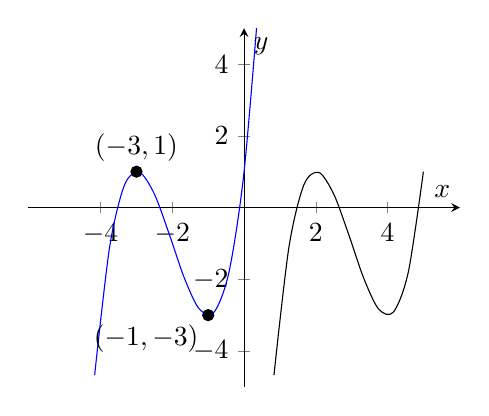
\begin{tikzpicture}[cmark/.style={label={[anchor=center]:\pgfuseplotmark{#1}}}]
			\begin{axis}
			[
				restrict y to domain=-10:10,
				restrict x to domain=-5:5,
				xlabel=$x$,
				ylabel=$y$,
				xmin=-5,
				xmax=5,
				xtick={-4,-2,...,4},
				ymin=-5,
				ymax=5,
				ytick={-4,-2,...,3},
				axis lines=center,
				axis equal,
				smooth,
				scale=0.8
			]
			\addplot [mark=none] {(x-3)^3-3*x+8};
			\addplot [color=blue,mark=none] {(x+2)^3-3*(x+5)+8};
			\coordinate
			[
				label=above:{$(-3,1)$},
				black,
				cmark=*,
			] (a) at (-3,1);
			\coordinate
			[
				label=below left:{$(-1,-3)$},
				black,
				cmark=*,
			] (a) at (-1,-3);
			\end{axis}
		\end{tikzpicture}
		\caption{$y=f(x+5)$ in blue, along with the original graph.}
	\end{subfigure}
	\caption{An example of a typical question about $y=f(x+a)$ with the solution.}
	\label{fig:horizontalShiftExample}
\end{figure}

To find out the transformed coordinates, add $-a$ to the $x$-coordinates:
\begin{align*}
f(x)&=(2,1) & f(x)&=(4,-3)\\
f(x+5)&=(-3,1) & f(x+5)&=(-1,-3)
\end{align*}


\section{Graph of $y=-f(x)$}
$y=-f(x)$ reflects the graph on the $x$-axis; all $y$-coordinates will change their sign.

An easy way to remember this is to think of the equation $y=x^2$ that was learnt in National 5. If the equation would be $y=-x^2$, then the parabola is ``flipped". This is the same thing that can be done to any function $y=f(x)$, $y=-f(x)$ will be ``flipped".

\subsection{Example}
An example of reflection on the $x$-axis with coordinates $(-1,3)$ and $(1,-1)$ is shown in figure \ref{fig:xAxisReflectionExample}.

\begin{figure}[h!]
	\centering
	\begin{subfigure}{0.475\linewidth}
		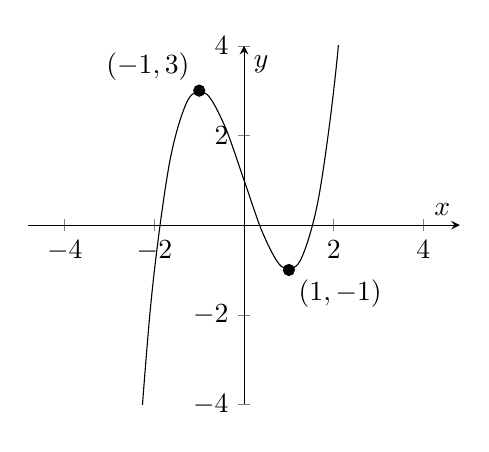
\begin{tikzpicture}[cmark/.style={label={[anchor=center]:\pgfuseplotmark{#1}}}]
			\begin{axis}
			[
				restrict y to domain=-10:10,
				restrict x to domain=-5:5,
				xlabel=$x$,
				ylabel=$y$,
				xmin=-4,
				xmax=4,
				xtick={-4,-2,...,4},
				ymin=-4,
				ymax=4,
				ytick={-4,-2,...,3},
				axis lines=center,
				axis equal,
				smooth,
				scale=0.8
			]
			\addplot [] {x^3-3*x+1};
			\coordinate
			[
				label=above left:{$(-1,3)$},
				black,
				cmark=*,
			] (a) at (-1,3);
			\coordinate
			[
				label=below right:{$(1,-1)$},
				black,
				cmark=*,
			] (a) at (1,-1);
			\end{axis}
		\end{tikzpicture}
		\caption{Some function $y=f(x)$ with a couple of given coordinates.}
	\end{subfigure}
	\begin{subfigure}{0.475\linewidth}
		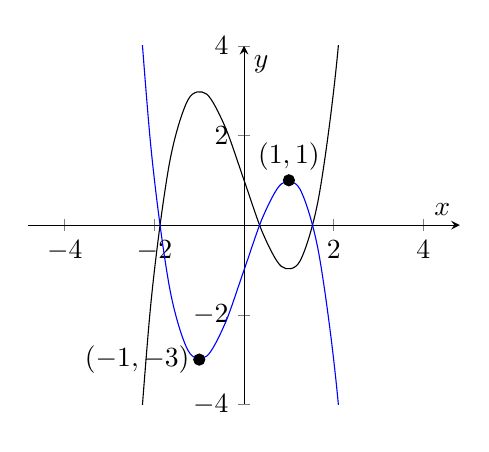
\begin{tikzpicture}[cmark/.style={label={[anchor=center]:\pgfuseplotmark{#1}}}]
			\begin{axis}
			[
				restrict y to domain=-10:10,
				restrict x to domain=-5:5,
				xlabel=$x$,
				ylabel=$y$,
				xmin=-4,
				xmax=4,
				xtick={-4,-2,...,4},
				ymin=-4,
				ymax=4,
				ytick={-4,-2,...,3},
				axis lines=center,
				axis equal,
				smooth,
				scale=0.8
			]
			\addplot [mark=none] {x^3-3*x+1};
			\addplot [color=blue,mark=none] {-x^3+3*x-1};
			\coordinate
			[
				label=left:{$(-1,-3)$},
				black,
				cmark=*,
			] (a) at (-1,-3);
			\coordinate
			[
				label=above:{$(1,1)$},
				black,
				cmark=*,
			] (a) at (1,1);
			\end{axis}
		\end{tikzpicture}
		\caption{$y=-f(x)$ in blue, along with the original graph.}
	\end{subfigure}
	\caption{An example of a typical question about $y=-f(x)$ with the solution.}
	\label{fig:xAxisReflectionExample}
\end{figure}

To find out the transformed coordinates, change the $y$-coordinates' sign:
\begin{align*}
	f(x)&=(-1,3) & f(x)&=(1,-1)\\
	-f(x)&=(-1,-3) & -f(x)&=(-1,-1)
\end{align*}


\section{Graph of $y=f(-x)$}
$y=f(-x)$ is reflection on the y-axis; all $x$-coordinates will change their signs.

\subsection{Example}
Here in figure \ref{fig:yAxisReflectionExample} an example of reflection on the $y$-axis is shown with the coordinates $(1,2)$ and $(3,-2)$.

\begin{figure}[h!]
	\centering
	\begin{subfigure}{0.475\linewidth}
		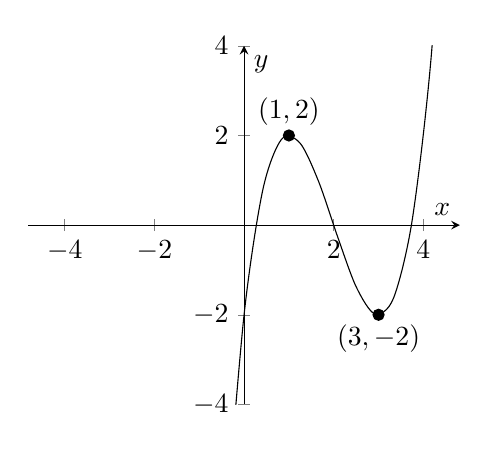
\begin{tikzpicture}[cmark/.style={label={[anchor=center]:\pgfuseplotmark{#1}}}]
			\begin{axis}
			[
				restrict y to domain=-10:10,
				restrict x to domain=-5:5,
				xlabel=$x$,
				ylabel=$y$,
				xmin=-4,
				xmax=4,
				xtick={-4,-2,...,4},
				ymin=-4,
				ymax=4,
				ytick={-4,-2,...,3},
				axis lines=center,
				axis equal,
				smooth,
				scale=0.8
			]
			\addplot [] {(x-2)^3-3*x+6};
			\coordinate
			[
				label=above:{$(1,2)$},
				black,
				cmark=*,
			] (a) at (1,2);
			\coordinate
			[
				label=below:{$(3,-2)$},
				black,
				cmark=*,
			] (a) at (3,-2);
			\end{axis}
		\end{tikzpicture}
		\caption{Some function $y=f(x)$ with a couple of given coordinates.}
	\end{subfigure}
	\begin{subfigure}{0.475\linewidth}
		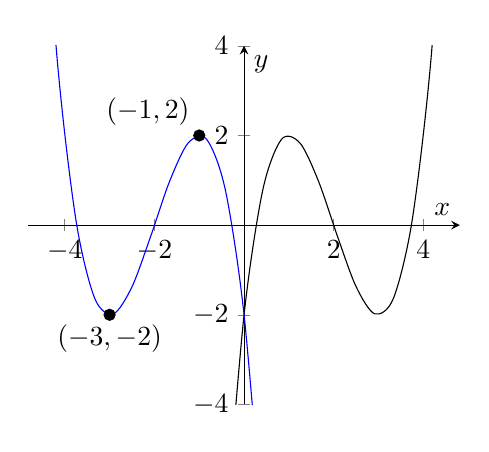
\begin{tikzpicture}[cmark/.style={label={[anchor=center]:\pgfuseplotmark{#1}}}]
			\begin{axis}
			[
				restrict y to domain=-10:10,
				restrict x to domain=-5:5,
				xlabel=$x$,
				ylabel=$y$,
				xmin=-4,
				xmax=4,
				xtick={-4,-2,...,4},
				ymin=-4,
				ymax=4,
				ytick={-4,-2,...,3},
				axis lines=center,
				axis equal,
				smooth,
				scale=0.8
			]
			\addplot [mark=none] {(x-2)^3-3*x+6};
			\addplot [color=blue,mark=none] {(-x-2)^3+3*x+6};
			\coordinate
			[
				label=above left:{$(-1,2)$},
				black,
				cmark=*,
			] (a) at (-1,2);
			\coordinate
			[
				label=below:{$(-3,-2)$},
				black,
				cmark=*,
			] (a) at (-3,-2);
			\end{axis}
		\end{tikzpicture}
		\caption{$y=f(-x)$ in blue, along with the original graph.}
	\end{subfigure}
	\caption{An example of a typical question about $y=f(-x)$ with the solution.}
	\label{fig:yAxisReflectionExample}
\end{figure}

To find out the transformed coordinates, change the $x$-coordinates' sign:
\begin{align*}
	f(x)&=(1,2) & f(x)&=(3,-2)\\
	f(-x)&=(-1,2) & f(-x)&=(-3,-2)
\end{align*}


\section{Graph of $y=kf(x)$}
A graph can be stretched or compressed on the $y$-axis by multiplying the graph by a constant, written as $y=kf(x)$. $k>1$ will stretch it, while $k<1$ will compress it.

To find out the new coordinates, multiply the $y$-coordinate by $k$.

\subsection{Example}
Figure \ref{fig:verticalCompressionExample} is the graph of $y=f(x)$, as well as $y=2f(x)$ and $y=\frac{1}{2}f(x)$.

\begin{figure}[h!]
	\centering
	\begin{subfigure}{0.475\linewidth}
		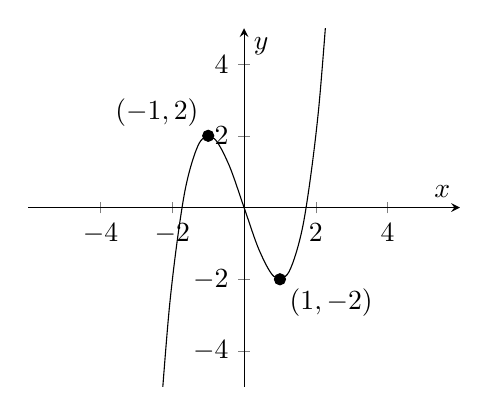
\begin{tikzpicture}[cmark/.style={label={[anchor=center]:\pgfuseplotmark{#1}}}]
			\begin{axis}
			[
				restrict y to domain=-10:10,
				restrict x to domain=-5:5,
				xlabel=$x$,
				ylabel=$y$,
				xmin=-5,
				xmax=5,
				xtick={-4,-2,...,4},
				ymin=-5,
				ymax=5,
				ytick={-4,-2,...,4},
				axis lines=center,
				axis equal,
				smooth,
				scale=0.8,
			]
			\addplot [] {x^3-3*x};
			\coordinate
			[
				label=above left:{$(-1,2)$},
				black,
				cmark=*,
			] (a) at (-1,2);
			\coordinate
			[
				label=below right:{$(1,-2)$},
				black,
				cmark=*,
			] (a) at (1,-2);
			\end{axis}
		\end{tikzpicture}
		\caption{Some function $y=f(x)$ with a couple of given coordinates.}
	\end{subfigure}
	\begin{subfigure}{0.475\linewidth}
		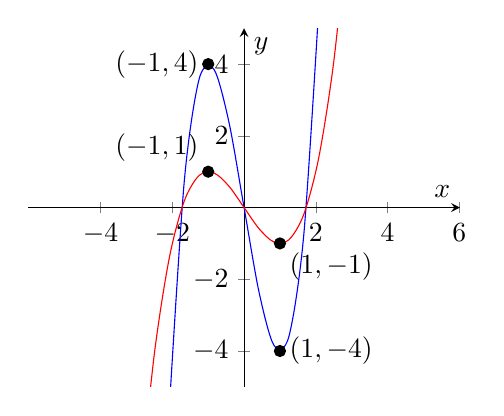
\begin{tikzpicture}[cmark/.style={label={[anchor=center]:\pgfuseplotmark{#1}}}]
			\begin{axis}
			[
				restrict y to domain=-10:10,
				restrict x to domain=-5:5,
				xlabel=$x$,
				ylabel=$y$,
				xmin=-5,
				xmax=5,
				xtick={-4,-2,...,5},
				ymin=-5,
				ymax=5,
				ytick={-4,-2,...,4},
				axis lines=center,
				axis equal,
				smooth,
				scale=0.8,
			]
			\addplot [color=blue,mark=none] {2*(x^3)-6*x};
			\addplot [color=red,mark=none] {0.5*(x^3)-1.5*x};
			\coordinate
			[
				label=left:{$(-1,4)$},
				black,
				cmark=*,
			] (a) at (-1,4);
			\coordinate
				[
				label=right:{$(1,-4)$},
				black,
				cmark=*,
			] (a) at (1,-4);
			\coordinate
			[
				label=above left:{$(-1,1)$},
				black,
				cmark=*,
			] (a) at (-1,1);
			\coordinate
			[
				label=below right:{$(1,-1)$},
				black,
				cmark=*,
			] (a) at (1,-1);
			\end{axis}
		\end{tikzpicture}
		\caption{$y=2f(x)$ in blue and $y=\frac{1}{2}f(x)$, original graph omitted for clarity.}
	\end{subfigure}
	\caption{An example of a typical question about $y=kf(x)$ with the solution.}
	\label{fig:verticalCompressionExample}
\end{figure}

To find out the transformed coordinates, multiply the $y$-coordinates by $k$. For $k=2$:
\begin{align*}
f(x)&=(-1,2) & f(x)&=(1,-2)\\
f(2x)&=(-1,4) & f(2x)&=(1,-4)
\end{align*}
And for $k=\frac{1}{2}$:
\begin{align*}
f(x)&=(-1,2) & f(x)&=(1,-2)\\
f\left(\frac{1}{2}x\right)&=(-1,1) & f\left(\frac{1}{2}x\right)&=(1,-1)
\end{align*}


\section{Graph of $y=f(kx)$}
The last transformation is stretching and compressing on the $x$-axis. Again, the opposite is true here, $k>1$ will \textit{compress} the graph, $k<1$ will stretch the graph.

To get the new coordinates, divide all $x$-coordinates by $k$.

\subsection{Examples}
Figure \ref{fig:horizontalCompressionExample} shows $y=f(x)$, and the graphs of $y=f(2x)$ and $y=f(\frac{1}{2})$.

\begin{figure}[h!]
	\centering
	\begin{subfigure}{0.475\linewidth}
		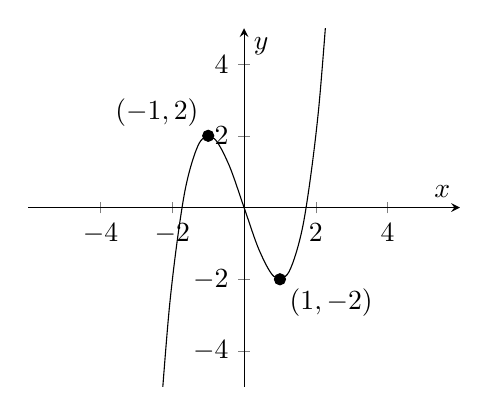
\begin{tikzpicture}[cmark/.style={label={[anchor=center]:\pgfuseplotmark{#1}}}]
			\begin{axis}
			[
				restrict y to domain=-10:10,
				restrict x to domain=-5:5,
				xlabel=$x$,
				ylabel=$y$,
				xmin=-5,
				xmax=5,
				xtick={-4,-2,...,4},
				ymin=-5,
				ymax=5,
				ytick={-4,-2,...,4},
				axis lines=center,
				axis equal,
				smooth,
				scale=0.8,
			]
			\addplot [] {x^3-3*x};
			\coordinate
			[
				label=above left:{$(-1,2)$},
				black,
				cmark=*,
			] (a) at (-1,2);
			\coordinate
			[
				label=below right:{$(1,-2)$},
				black,
				cmark=*,
			] (a) at (1,-2);
			\end{axis}
		\end{tikzpicture}
		\caption{Some function $y=f(x)$ with a couple of given coordinates.}
	\end{subfigure}
	\begin{subfigure}{0.475\linewidth}
		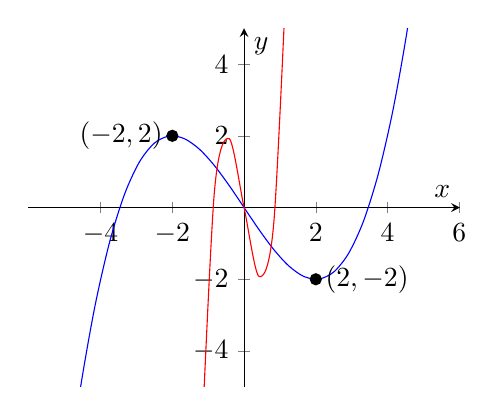
\begin{tikzpicture}[cmark/.style={label={[anchor=center]:\pgfuseplotmark{#1}}}]
			\begin{axis}
			[
				restrict y to domain=-10:10,
				restrict x to domain=-5:5,
				xlabel=$x$,
				ylabel=$y$,
				xmin=-5,
				xmax=5,
				xtick={-4,-2,...,5},
				ymin=-5,
				ymax=5,
				ytick={-4,-2,...,4},
				axis lines=center,
				axis equal,
				smooth,
				scale=0.8,
			]
			\addplot [color=blue,mark=none] {(x/2)^3-1.5*x};
			\addplot [color=red,mark=none] {(2*x)^3-6*x};
			\coordinate
			[
				label=left:{$(-2,2)$},
				black,
				cmark=*,
				] (a) at (-2,2);
			\coordinate
			[
				label=right:{$(2,-2)$},
				black,
				cmark=*,
			] (a) at (2,-2);
			\end{axis}
		\end{tikzpicture}
		\caption{$y=f(\frac{1}{2}x)$ in blue and $y=f(2x)$ in red, original graph and coordinates of $y=f(\frac{1}{2}x)$ omitted for clarity.}
	\end{subfigure}
	\caption{An example of a typical question about $y=f(kx)$ with the solution.}
	\label{fig:horizontalCompressionExample}
\end{figure}

To find out the transformed coordinates, divide the $x$-coordinates by $k$. For $k=\frac{1}{2}$:
\begin{align*}
f(x)&=(-1,2) & f(x)&=(1,-2)\\
f(2x)&=(-2,2) & f(2x)&=(2,-2)
\end{align*}
And for $k=2$:
\begin{align*}
f(x)&=(-1,2) & f(x)&=(1,-2)\\
f\left(\frac{1}{2}x\right)&=\left(-\frac{1}{2},2\right) & f\left(\frac{1}{2}x\right)&=\left(\frac{1}{2},-1\right)
\end{align*}
\addtocontents{toc}{\setcounter{tocdepth}{3}}
\chapter{Differentiation}
\section{What Is Differentiation?}

\textbf{None of this section on what differentiation has to be known for the exam (except for the notation), though it's incredibly useful to know.}

\subsection{Understanding Rate of Change}
To measure how much something has changed, the difference can be found. For example, look at the following graph of the EUR/USD price from January to December 2019.

\begin{figure}[h!]
	\centering
	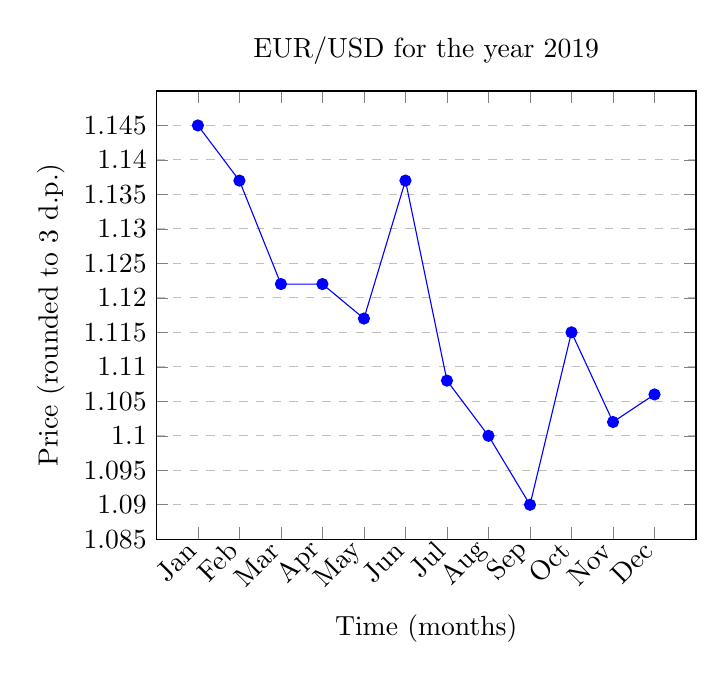
\begin{tikzpicture}
	\begin{axis}
	[
		title={EUR/USD for the year 2019},
		xlabel={Time (months)},
		ylabel={Price (rounded to 3 d.p.)},
		xmin=0,
		xmax=13,
		xtick={0,1,...,12},
		xticklabels={ ,Jan, Feb, Mar, Apr, May, Jun, Jul, Aug, Sep, Oct, Nov, Dec},
		ymin=1.085,
		ymax=1.150,
		ytick={1.085,1.090,...,1.145},
		x tick label style= {rotate=45, anchor=east},
		ymajorgrids=true,
		grid style=dashed,
		/pgf/number format/precision=3,
	]
		\addplot
		[
			color=blue,
			mark=*,
		] coordinates
		{
			(1,1.145) (2,1.137) (3,1.122) (4,1.122) (5,1.117) (6,1.137) (7,1.108) (8,1.100) (9,1.090) (10,1.115) (11,1.102) (12,1.106)
		};
	\end{axis}
	\end{tikzpicture}
	\caption{The EUR/USD course for January to December in 2019, rounded to 3 decimal places.}
	\label{fig:EURUSD}
\end{figure}

The change of the graph between December and January is the difference in their values. The exact values of those months are $1.145$ and $1.106$, so
\begin{align*}
	\text{difference in price} &= 1.145 - 1.106\\
	&=0.039\text{.}
\end{align*}

The rate of change is how quickly something changes, or in other words, the change that is experienced over time. The rate of change between January and December would be found by dividing the change by the time taken.

\begin{align*}
	\frac{\text{difference in price}}{\text{difference in time}} &=\frac{1.145-1.106}{12-1}\\[0.75em]
	&=\frac{0.039}{11} \approx 3.55\times10^{-3}
\end{align*}

More generally, the rate of change between any $x$ and $y$ is the difference in $y$ over the difference in $x$.
\begin{align*}
\text{rate of change} &= \frac{\text{difference in $y$}}{\text{difference in $x$}}
\end{align*}

\subsection{Paradox of the Instantaneous Rate of Change}
Suppose we would graph the distance over time of a quick vehicle. For reasons that'll become more clear later on, the symbol $s$ is used for displacement instead of distance. This graph just so happens to be the graph of $d=t^2$, how convenient!

\begin{figure}[h!]
	\centering
	\begin{tikzpicture}
		\begin{axis}
		[
			restrict y to domain=0:25,
			restrict x to domain=0:5,
			xlabel=$t (s)$,
			ylabel=$d (m)$,
			xmin=0,
			xmax=5,
			xtick={0,1,...,4},
			ymin=0,
			ymax=17,
			ytick={0,2,...,16},
			axis lines=center,
			smooth,
			samples=50
		]
		\addplot [color=black,mark=none] {x^2};
		\end{axis}
	\end{tikzpicture}
	\caption{Displacement ($s$) in metres over time ($t$) in seconds.}
	\label{POIexample}
\end{figure}

The vehicle starts slowly and quickly begins to travel faster and faster. It would be very helpful to know how quick the car is going at a time of, say, 3 seconds. In other words, it would be helpful to know its instantaneous rate of change at 3 seconds (remember, rate of change is the change in value over time, in this case it's the change in displacement over time, the velocity).

The problem is that there is no such thing as "instantaneous" rate of change. To have a rate of change, there must be a time that has elapsed. That's not very helpful though, there must be a way to find out how quick the car is going --- its velocity (symbol $v$) --- at in a moment in time.

The solution to this is to decrease the change in time that's being used until it's nearly $0$, as close to $0$ as you could get. By coming closer and closer to 0, a certain value is approached. Let's try using a change in time of 3.1 and 3.01 and see what happens.

\begin{align*}
	v&=\frac{\text{difference in $d$}}{\text{difference in $t$}} & v&=\frac{\text{difference in $d$}}{\text{difference in $t$}}\\[0.75em]
	v &= \frac{9.61-9}{3.1-3} & v &= \frac{9.0601-9}{3.01-3}\\
	&= 6.1 & &= 6.01
\end{align*}

As you can see, a value of $6$ is approached whenever a smaller value for the change in time is taken. As previously said, there is no such thing as instantaneous change, but instead the best approximation can be calculated. In this case, the best approximation for the rate of change can be concluded to be $6$.

That is what the derivative is. The best approximation for the rate of change.

Whenever the difference in the values will approach $0$, the symbol $d$ can be used, so more generally you can write for any $x$ and $y$,
\begin{equation}
	\text{derivative} = \frac{dy}{dx}\text{.}
\end{equation}

\subsection{Notation}
When an equation (such as $d=t^2$ like above) is differentiated, it is done with respect to one variable. Usually, equations are in the form $y=x$ where there might be lots on the $x$ side, but little on the $y$ side. When such an equation is differentiated, it is said to have been done ``with respect to x". The above example was differentiated with respect to $t$.

There are numerous ways of writing the derivative, each having a good use in different fields. In maths, two ways of writing the derivative are used: the one used by Leibniz, one of the independent discoverers of calculus, and the one used by Lagrange.

\subsubsection{Leibniz's Notation}
Leibniz notation is actually the one that has been used so far. The derivative of two variables $x$ and $y$ can be written as $\frac{dy}{dx}$ and is read out ``the derivative of $y$ with respect to $x$.
\subsection{Lagrange's Notation}
However, sometimes a function has to be differentiated. For example, the derivative of $f(x) = 6x^3$ is $18x^2$, but how is that written? A prime mark is added between the $f$ and $x$, and it is read as ``the derivative evaluated at $x$".
\begin{align*}
	f(x) &= 6x^3\\
	f'(x) &= 18x^2
\end{align*}


\section{A Shortcut to Differentiate}
Doing the above is very tedious, so luckily there is a shortcut that can be taken! Multiply the coefficient of the variable by the power, and subtract $1$ from the power. More formally,
\begin{align*}
	f(x) &= x^n\\
	f'(x) &= nx^{n-1}
\end{align*}

This is called the ``power rule".

\subsection{Examples}
Note that it's not required to continue to simplify after the derivative is found, however it might be helpful in more complex questions.

\begin{enumerate}
	\item
	\begin{align*}
		f(x) &= 5x^5\\
		f'(x) &= 25x^4
	\end{align*}
	\item
	\begin{align*}
		f(x) &= \frac{2}{x}\\
		&= x^{-2}\\
		f'(x) &= -2x^{-3}\\
		&= \frac{-2}{x^3}
	\end{align*}
	\item 
	\begin{align*}
		f(x) &= \frac{3}{\sqrt[4]{x^2}}\\
		&= \frac{3}{x^{\frac{2}{4}}}\\
		&= 3x^{-\frac{2}{4}}\\
		f'(x) &= -\frac{14}{4}x^{-\frac{6}{4}}\\[0.5em]
		&= \frac{-\frac{14}{4}}{x^{\frac{6}{4}}}\\[0.5em]
		&= \frac{-\frac{14}{4}}{\sqrt[4]{x^6}}
	\end{align*}
\end{enumerate}
\addtocontents{toc}{\setcounter{tocdepth}{2}}
\chapter{Integration}
Integration is the opposite to differentiation. While differentiation is finding the tangent to a line, integration is finding the area under this line (usually called ``area under the graph").

\section{What Is Integration?}
Suppose a car is decelerating and the velocity-time graph of this car is conveniently the equation $v=-\left(t^2\right)+4$ as shown.

\begin{figure}[h!]
	\centering
	\begin{tikzpicture}
		\begin{axis}
		[
			restrict y to domain=0:6,
			restrict x to domain=0:3,
			xlabel=$t\ (s)$,
			ylabel=$v\ (m\ s^{-1})$,
			xmin=0,
			xmax=3,
			xtick={0,1,2},
			ymin=0,
			ymax=5,
			ytick={0,1,...,4},
			axis lines=center,
			smooth,
			samples=150
		]
			\addplot [color=black,mark=none] {-x^2+4};
		\end{axis}
	\end{tikzpicture}
	\caption{The curve of a car decelerating.}
	\label{fig:integrationBasicEx1}
\end{figure}

How can the distance (referred to as ``displacement", symbol $s$) that the car has travelled during this time be found? From a velocity-time graph, the displacement travelled is the area under the graph.

Note how finding the derivative is finding the ``higher" level; for a travelling car it the derivative of the distance over time is the speed, and the derivative of the velocity over time is the acceleration. When integrating, the ``lower" level is found; so the integral of the acceleration becomes the velocity, and the integral of the velocity is the displacement.

One way to find the area under the graph (and therefore the displacement travelled) is to approximate it using a rectangle (blue in figure \ref{fig:integrationBasicEx2}). This will give an okay estimate, but not a very accurate one. The area can be found as shown.

\begin{figure}[h!]
	\centering
	\begin{tikzpicture}
	\begin{axis}
	[
		restrict y to domain=0:6,
		restrict x to domain=0:3,
		xlabel=$t\ (s)$,
		ylabel=$v\ (m\ s^{-1})$,
		xmin=0,
		xmax=3,
		xtick={0,1,2},
		extra x ticks={0},
		ymin=0,
		ymax=5,
		ytick={0,1,...,4},
		extra y ticks={0},
		axis lines=center,
		smooth,
		samples=150
	]
		\addplot [color=black,mark=none] {-x^2+4};
		\addplot [color=blue,mark=none,domain=0:2] {4};
		\addplot [color=blue,mark=none,domain=0:2] {0};
		\addplot [color=blue,mark=none] coordinates {(2,0) (2,4)};
		\addplot [color=blue,mark=none] coordinates {(0,0) (0,4)};
	\end{axis}
	\end{tikzpicture}
	\caption{In blue is an approximation for the area.}
	\label{fig:integrationBasicEx2}
\end{figure}

\begin{align*}
	s&=\text{area under graph}\\
	s&=\text{length} \cdot \text{height}\\
	s&=2 \cdot 4\\
	s&=8 \text{ m}
\end{align*}

How could the area under the graph be found in an even more accurate way? More rectangles can be drawn as shown in figure \ref{fig:integrationBasicEx3}. Instead of using a time interval of $2$, a smaller interval could be used. For example, suppose that the differences in time are $0.5$ and not $2$ like before. $t=0.5$ is drawn until it touches the graph. The same is done for $t=1.0$, $t=1.5$, and $t=2.0$ to give four rectangles as shown. This is quite a bit more accurate than using just one rectangle.

\begin{figure}[h!]
	\centering
	\begin{tikzpicture}
	\begin{axis}
	[
		restrict y to domain=0:6,
		restrict x to domain=0:3,
		xlabel=$t\ (s)$,
		ylabel=$v\ (m\ s^{-1})$,
		xmin=0,
		xmax=3,
		xtick={0,0.5,...,2},
		extra x ticks={0},
		ymin=0,
		ymax=5,
		ytick={0,0.25,...,4},
		yticklabels={0,,0.5,,1,,1.5,,2,,2.5,,3,,3.5,,4},
		extra y ticks={0},
		axis lines=center,
		smooth,
		samples=150
	]
		\addplot [color=black,mark=none] {-x^2+4};
		\addplot [color=blue,mark=none,domain=0.0:0.5] {4};
		\addplot [color=blue,mark=none,domain=0.5:1.0] {3.75};
		\addplot [color=blue,mark=none,domain=1.0:1.5] {3};
		\addplot [color=blue,mark=none,domain=1.5:2.0] {1.75};
		\addplot [color=blue,mark=none,domain=0.0:2.0] {0};
		\addplot [color=blue,mark=none] coordinates {(2,0) (2,1.75)};
		\addplot [color=blue,mark=none] coordinates {(1.5,0) (1.5,3)};
		\addplot [color=blue,mark=none] coordinates {(1,0) (1,3.75)};
		\addplot [color=blue,mark=none] coordinates {(0.5,0) (0.5,4)};
		\addplot [color=blue,mark=none] coordinates {(0,0) (0,4)};
	\end{axis}
	\end{tikzpicture}
	\caption{In blue is a more accurate approximation for the area.}
	\label{fig:integrationBasicEx3}
\end{figure}

To figure out the area of figure \ref{fig:integrationBasicEx3}, the area of the four rectangles would be found as shown below.

\begin{align*}
	s&=\text{area under graph}\\
	s&=0.5 \cdot 4 + 0.5 \cdot 3.75 + 0.5 \cdot 3 + 0.5 \cdot 1.75\\
	s&=6.25 \text{ m}
\end{align*}

By using smaller differences in time, a more accurate value can be gotten. When this difference in time gets smaller, more rectangles need to be added together. It's almost like a bunch of sums. Eventually, the width of those rectangles will be, eventually the width will be so small that it's negligible. So it can be assumed that the area is just its height, as when $A = \text{length} \cdot \text{height}$ and length becomes negligible, area becomes $A = \text{height}$.

In other words, to work out the area under the graph, the heights of all the rectangles can be multiplied by whatever difference in time we chose (the ``width") and added together. However, the difference in time becomes so small that it becomes negligible.

This is written formally as
\begin{equation*}
	\int_{0}^{2} -t^2+4 \, dt
\end{equation*}
where:
\begin{itemize}
	\item the weird S sign is the integral symbol (it looks like an S for sum, since a lot of rectangles are summed together),
	\item the little $0$ and $2$ show where the start and end-points of the function are (see how in our above examples time only went from $0$ to $2$ seconds), this is called the lower-bound and upper-bound respectively,
	\item the $-x^2+4$ is whatever formula we chose to have,
	\item and the $dt$ stands for the difference in time that we eventually let approach to 0. Note leaving out that this and the constant of integration (covered later) are the two most often made mistakes, so definitely check that you've included them at the end of an exam!
\end{itemize}

More on areas under graphs is explained in a later chapter, focussing on further examples on finding areas under graphs and showing how you can actually use integrals to find the exact area.

\section{Indefinite Integrals}
Integrals without any lower- or upper-bounds are called indefinite integrals. This is also called doing ``antidifferentiation", as it's essentially the opposite of differentiating.

To integrate, raise the variable's power by $1$ and then divide the variable with its coefficient by the new raised power. In other words,
\begin{align}
	&\int x^n \, dx\\
	&= \frac{x^{(n+1)}}{n+1}\text{.}
\end{align}

\subsection{The Constant of Integration}
When differentiating an expression such as $f(x) = 2x^2+5$, the $5$ gets lost and all that's left is $f'(x) = 4x$. So when integrating $4x$ all that can be gotten is $\int 4x \, dx = 2x^2$. Notice that $5$ cannot be gotten back out. Therefore any indefinite integral must include the constant of integration, a $+C$.

Why is this not needed for a definite integral? Well, since two different integrals are subtracted, the two $+C$s will cancel, so it can just be left out.

\addtocontents{toc}{\setcounter{tocdepth}{1}}
\subsection{Examples}
\begin{enumerate}
	\item
	\begin{align*}
		&\int x^2 \, dx\\
		&= \frac{x^3}{3} + C
	\end{align*}
	
	\item
	\begin{align*}
		&\int 4x^3 \, dx\\
		&= \frac{4x^4}{4} + C\\
		&= x^4+C
	\end{align*}
	
	\item
	\begin{align*}
		&\int 9 \, dx\\
		&= 9x + C
	\end{align*}
	
	\item
	\begin{align*}
		&\int \left(x^2+x^{-7}\right) \, dx\\
		&= \frac{x^3}{3} + \frac{x^{-6}}{-6} + C\\
		&= \frac{x^3}{3} + \frac{1}{-6x^6} + C\\
		&= \frac{x^3}{3} - \frac{1}{6x^6} + C
	\end{align*}
\end{enumerate}

\section{Definite Integrals (Finding Areas Under (or Over) Graphs)}
When finding the area under a graph between two points, the integral of the graph between the two points can be found. The integral of figure \ref{fig:integralDefiniteEx1} is as shown.
\begin{figure}[h!]
	\centering
	\begin{tikzpicture}
	\begin{axis}
	[
		restrict y to domain=0:25,
		restrict x to domain=0:5,
		xlabel=$x$,
		ylabel=$y$,
		xmin=0,
		xmax=5.5,
		xticklabels={,,,$a$,$b$,},
		extra x ticks={0},
		ymin=0,
		ymax=16,
		yticklabels={,,,,},
		extra y ticks={0},
		axis lines=center,
		smooth,
		samples=150
	]
		\addplot [color=black,mark=none,name path=y] {(x-1)^2};
		\path [name path = xaxis] (axis cs:2,0) -- (axis cs:3,0);
		\addplot [pattern=north west lines,pattern color=blue] fill between[of=y and xaxis, soft clip={domain=2:3}];
		\addplot [color=blue,mark=none,dashed] coordinates {(2,0) (2,1)};
		\addplot [color=blue,mark=none,dashed] coordinates {(3,0) (3,4)};
	\end{axis};
	\end{tikzpicture}
	\caption{The hatched area is what is to be found.}
	\label{fig:integralDefiniteEx1}
\end{figure}
\begin{equation}
	\int_{a}^{b} f(x) dx
\end{equation}

If the antiderivative of $f(x)$ is given the variable $F(x)$, then the fundamental theorem of calculus can be described as shown.

\begin{equation}
	\int_{a}^{b} f(x) \, dx = F(b) - F(a)
\end{equation}

In other words, once the antiderivative is found, substitute $x$ for $a$ and subtract it by the antiderivative with $x$ substituted for $b$.

The notation for subtracting two antiderivatives is shown in the examples below; seeing it is often easier to understand than reading it.

\subsection{Examples}
\begin{enumerate}
	\item
	The graph of the function $y=x^2+2x$ is sketched in figure \ref{fig:integralDefiniteEx2}. Find the area of the shaded part of the graph.
	\begin{figure}[h!]
		\centering
		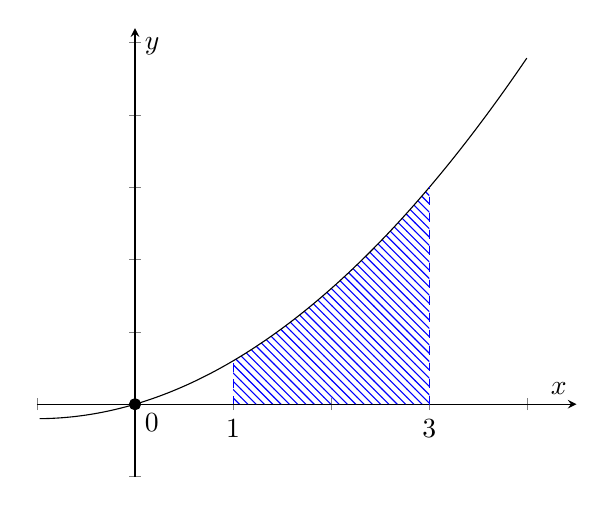
\begin{tikzpicture}[cmark/.style={label={[anchor=center]:\pgfuseplotmark{#1}}}]
			\begin{axis}
			[
				restrict y to domain=-5:25,
				restrict x to domain=-1:4,
				xlabel=$x$,
				ylabel=$y$,
				xmin=-1,
				xmax=4.5,
				xtick={-1,0,...,4},
				xticklabels={,,1,,3},
				ymin=-5,
				ymax=26,
				ytick={-5,0,...,25},
				yticklabels={,,,,,,,},
				axis lines=center,
				smooth,
				samples=150
			]
				\addplot [color=black,mark=none,name path=y] {x^2+2*x};
				\path [name path = xaxis] (axis cs:1,0) -- (axis cs:3,0);
				\addplot [pattern=north west lines,pattern color=blue] fill between[of=y and xaxis, soft clip={domain=1:3}];
				\addplot [color=blue,mark=none,dashed] coordinates {(1,0) (1,3)};
				\addplot [color=blue,mark=none,dashed] coordinates {(3,0) (3,15)};
				\coordinate [label=below right:{$0$},black,cmark=*] (o) at (0,0);
			\end{axis};
		\end{tikzpicture}
		\caption{Graph of $y=x^2+2x$, not to scale.}
		\label{fig:integralDefiniteEx2}
	\end{figure}
	
	\item
	Find the positive value of $Z$ for which $\int_{1}^{Z} (1+2x) \, dx = 4$
\end{enumerate}

\begin{enumerate}
	\item
	\begin{align*}
		&\int_{1}^{3} (x^2 + 2x) \, dx\\
		&=\left[ \frac{x^3}{3} + \frac{2x^2}{2} \right]_1^3\\
		&=\left[ \frac{x^3}{3} + x^2 \right]_1^3\\
		&=\left[ \frac{3^3}{3} + 3^2 \right] - \left[ \frac{1^3}{3} + {1^2} \right]\\
		&= \left[ 18 \right] - \left[ \frac{4}{3} \right]\\
		&= \frac{50}{3} \text{ units}^2
	\end{align*}
	Note that the units is squared, as an area is found.
	
	\item
	\begin{align*}
		\int_{1}^{Z} (1+2x) \, dx &= 4\\
		\left[ x+x^2 \right]_1^Z &= 4\\
		\left[ Z+Z^2 \right] - \left[ 1+1^2 \right] &= 4\\
		Z+Z^2 - 2 &= 4\\
		Z^2+Z - 6 &= 0\\
		\left(Z+3\right)\left(Z-2\right) &= 0\\
	\end{align*}
	\begin{align*}
		&Z=-3 & Z&=2\\
		&\text{Disregard, as $Z$ must be positive.} & &
	\end{align*}
\end{enumerate}

\section{Working With Negative Area}
Integrating a graph which goes below the $x$-axis will give a negative area. Is this useful?

Using the car example, the graph goes below the $x$-axis when it goes backwards. If the total displacement is to be found then yes, it's very helpful. But the total distance that the car drove would always be positive.

Generally in maths, when you have to find an area under a graph that goes into the negative then you must change a negative area to a positive one.

\subsection{Examples}
\begin{enumerate}
	\item
	Find the area under the graph of $f(x) = 2x+4$ between $x=-2$ and $x=2$.
	
	\item
	Figure \ref{fig:integralNegativeAreaEx1} shows the graph of $y=8-2x-x^2$. Find the area of the graph between $x=-5$ and $x=2$.
\end{enumerate}

\begin{figure}[h!]
	\centering
	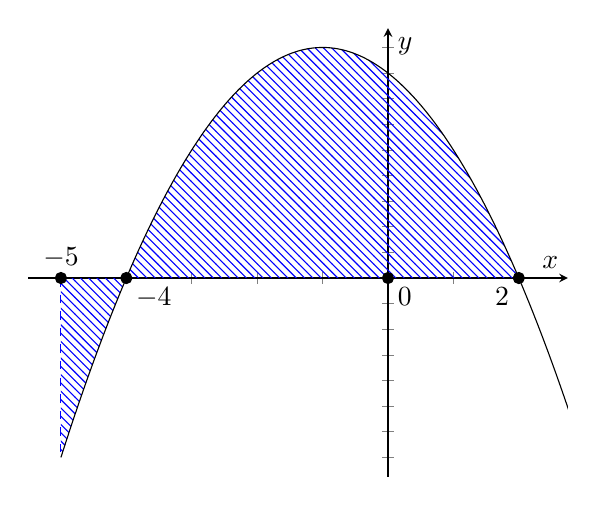
\begin{tikzpicture}[cmark/.style={label={[anchor=center]:\pgfuseplotmark{#1}}}]
		\begin{axis}
		[
			restrict y to domain=-7.75:9.5,
			restrict x to domain=-5.5:9,
			xlabel=$x$,
			ylabel=$y$,
			xmin=-5.5,
			xmax=2.75,
			xtick={-5,-4,...,2},
			xticklabels={,,},
			ymin=-7.75,
			ymax=9.75,
			ytick={-7,-6,...,9},
			yticklabels={,,},
			axis lines=center,
			smooth,
			samples=75
		]
			\addplot [color=black,mark=none,name path=y] {8-2*x-x^2};
			\path [name path = xaxis] (axis cs:-5,0) -- (axis cs:2,0);
			\addplot [pattern=north west lines,pattern color=blue] fill between[of=y and xaxis, soft clip={domain=-5:2}];
			\addplot [color=blue,mark=none,dashed] coordinates {(-5,0) (-5,-7)};
			\coordinate [label=below right:{$0$},black,cmark=*] (o) at (0,0);
			\coordinate [label=above:{$-5$},black,cmark=*] (a) at (-5,0);
			\coordinate [label=below right:{$-4$},black,cmark=*] (b) at (-4,0);
			\coordinate [label=below left:{$2$},black,cmark=*] (c) at (2,0);
		\end{axis};
	\end{tikzpicture}
	\caption{Graph of $y=8-2x-x^2$, not to scale.}
	\label{fig:integralNegativeAreaEx1}
\end{figure}

\begin{enumerate}
	\item
	\begin{align*}
		&\int_{-2}^{2} 2x-4 \, dx\\
		&=\left[ x^2-4x \right]_{-2}^2\\
		&=\left[ 2^2-4\left(2\right) \right] - \left[ \left(-2\right)^2-4\left(-2\right) \right]\\
		&=-4-12\\
		&=-16 \text{ units}^2
	\end{align*}
	As the area must be positive, the area is $16$ units$^2$.
	
	\item
	$A_{\text{total}} = A_{\text{below}} + A_{\text{above}}$
	\begin{align*}
		A_{below} &= \int_{-5}^{-4} (8-2x-x^2) dx\\
		&= \left[ 8x-x^2-\frac{x^3}{3} \right]_{-5}^{-4}\\
		&= \left[ 8\left(-4\right) - \left(-4\right)^2 - \frac{(-4)^3}{3} \right] - \left[ 8\left(-5\right) - \left(-5\right)^2 - \frac{(-5)^3}{3} \right]\\
		&= \left[ -32-16 + \frac{64}{3} \right] - \left[ -40-25 + \frac{125}{3} \right]\\
		&= \left[ -\frac{80}{3} \right] - \left[ -\frac{80}{70}\right]\\
		&= -\frac{10}{3} \text{ units}^2
	\end{align*}
	However, area is positive, so $A_{below} = \frac{10}{3}$ units$^2$.
	
	\begin{align*}
		A_{above} &= \int_{-4}^{2} (8-2x-x^2) dx\\
		&= \left[ 8x-x^2-\frac{x^3}{3} \right]_{-4}^{2}\\
		&= \left[ 8\left(2\right) - \left(2\right)^2 - \frac{(2)^3}{3} \right] - \left[ 8\left(-4\right) - \left(-4\right)^2 - \frac{(-4)^3}{3} \right]\\
		&= \left[ 16-4 - \frac{8}{3} \right] - \left[ -32-16 + \frac{64}{3} \right]\\
		&= \left[ \frac{28}{3} \right] - \left[ -\frac{80}{3}\right]\\
		&= \frac{28}{3} + \frac{80}{3}\\
		&= 36 \text{ units}^2
	\end{align*}
	
	\begin{align*}
		A_{\text{total}} &= A_{\text{below}} + A_{\text{above}}\\
		&= \frac{10}{3} + 36\\
		&= \frac{10+108}{3}\\
		&= \frac{118}{3}\\
		&= 39\frac{1}{3} \text{ units}^2
	\end{align*}
\end{enumerate}
\chapter{Skills from National 5}

\section{Distance Formula}
The Distance Formula allows us to find the distance between two points given their Cartesian coordinates. To do this we treat the line between the two points as though it were the hypotenuse of a right-angled triangle, and use Pythagoras' theorem to find the length of the hypotenuse.

DIAGRAM GOES HERE.

To find each side we simply take the difference between the two $x$-coordinates $y$-coordinates, and substitute into Pythagoras' theorem.

Pythagoras' theorem:
\begin{equation*}
	a^2 = b^2+c^2
\end{equation*}

Rearranged, with our method to find the distances:
\begin{equation*}
	d = \sqrt{(x_2-x_1)^2+(y_2-y_1)^2}
\end{equation*}

\section{Completing the Square}
Completing the square is turning a quadratic from the form $ax^2 + bx + c$ to the form $p(x + q)^2+r$. There are multiple ways to do this, all of which will use the example quadratic $2x^2-6x+77$.

\subsection{Method 1 — Substitution}
The question will always give the completed square form, that is $p(x - q)^2+r$ (though the variables might be different ones, like $a$, $b$, $c$, or so). This can be expanded, as shown.
\begin{align*}
	&p(x+q)^2+r\\
	&p(x^2+2qx+q^2)+r\\
	&px^2+2pqx+pq^2+r
\end{align*}
It can be seen that $a$ became $p$, $b$ became $2pq$, and $c$ became $pq^2+r$. From there, a series of equations can be made and solved (practically this is done from left to right as shown).
\begin{align*}
	p &= a & 2pq &= b         & pq^2+r &= c\\
	p &= 2 & 2 \cdot 2q &=-24 & 2 \cdot (-6)^2 + r &= 77\\
	  &    & 4q &= -24        & 2 \cdot 36 + r &= 77\\
	  &    & q &= -6          & 72 + r &= 77\\
	  &    & &                & r &= 77 - 72\\
	  &    & &                & r &= 5
\end{align*}
Now that $p$, $q$, and $r$ have been found, they can be substituted back into completed square form.
\begin{equation*}
	2x^2-24x+77 = 2(x-6)^2+5
\end{equation*}

\subsection{Method 2 — Halving the Coefficient $b$}
When $a=1$, in the form $p(x+q)^2+r$, $q$ will be half of $b$. Using this fact a perfect square can be created. However, this will (almost) always give an incorrect value for $c$; the constant $r$ corrects this issue.

In other words, first, halve $b$ to find $q$. Then multiply the expression out and compare the $c$ that is gotten with the $c$ in the question. Finally, correct the discrepancy.

In $2x^2-24x+77$, the quadratic has to be partially factorised, factoring the first two terms. This must be done so that $a=1$, even if this gives a fractional $b$.
\begin{align*}
	&2x^2-24x+77\\
	&=2(x^2-12x)+77
\end{align*}
Next, $b$ is halved.
\begin{equation*}
	-12 \div 2 = -6
\end{equation*}
Now part of the final square form can be written.
\begin{equation*}
	2(x-6)^2
\end{equation*}
But this isn't the final solution. It must be multiplied out to see what value for $c$ is received. This will be the square of $b$ multiplied by whatever was factored out.
\begin{align*}
	&2(x-6)^2\\
	&=2x^2-24x+72
\end{align*}
Since $c$ is actually $77$ it can be deduced that a further $5$ is needed ($77-72=5$), which gives the final answer.
\begin{equation*}
	2x^2 - 24x + 77 = 2(x-6)^2+5
\end{equation*}

\section{Rationalising the Denominator}
When a fraction uses an irrational number as its denominator it can be difficult to understand what it's actually quantifying (try to imagine 5 $\sqrt(2)$ pieces of pizza!). Instead, the denominator can be rationalised. This has to be done in the final answer to an exam question, but isn't necessary (and sometimes even unhelpful) to be done mid-question.

When the denominator contains a root, the whole fraction should be multiplied by one in the form of this root.
\begin{align*}
	&\frac{5}{\sqrt{2}}\\
	&=\frac{5}{\sqrt{2}} \cdot \frac{\sqrt{2}}{\sqrt{2}}\\
	&=\frac{5\sqrt{2}}{\sqrt{2}\sqrt{2}}\\
	&=\frac{5\sqrt{2}}{2}
\end{align*}
And that is all there is to it, simply multiply the fraction by whatever root the denominator has. Here's another example.
\begin{align*}
	&\frac{300\sqrt{2}}{5\sqrt{40}}\\[5pt]
	&=\frac{300\sqrt{2}}{5\sqrt{4 \cdot 10}}\\[5pt]
	&=\frac{300\sqrt{2}}{5 \cdot 2\sqrt{10}}\\[5pt]
	&=\frac{300\sqrt{2}}{10\sqrt{10}}\\[5pt]
	&=\frac{30\sqrt{2}}{\sqrt{10}}\\[5pt]
	&=\frac{30\sqrt{2}}{\sqrt{10}} \cdot \frac{\sqrt{10}}{\sqrt{10}}\\[5pt]
	&=\frac{30\sqrt{2}\sqrt{10}}{\sqrt{10}\sqrt{10}}\\[5pt]
	&=\frac{30\sqrt{2}\sqrt{10}}{10}\\[5pt]
	&=3\sqrt{2}\sqrt{10}\\
	&=3\sqrt{20}\\
	&=3\sqrt{4 \cdot 5}\\
	&=3 \cdot 2 \sqrt{5}\\
	&=6\sqrt{5}
\end{align*}

\backmatter
% bibliography, glossary and index would go here.

\end{document}